\documentclass{article}
\usepackage{amsmath,amsthm,amssymb}
\usepackage{mathtext}
\usepackage[T2A]{fontenc}
\usepackage[utf8]{inputenc}
\usepackage[english]{babel}
\usepackage{graphicx}
\usepackage{hyperref}
\usepackage{mathtools}
\usepackage{multirow}

\title{STONKS - Stock Market Forecasting Using News Articles With Reinforcement And Sequence Learning}
\author{Ruslan Sirazhetdinov} 

\date{May 2023}



\begin{document}
\maketitle
\begin{abstract}
    I believe, that there is a correlation between price change direction of a particular share and news articles. The purpose of this project is to predict market price for next day, each time depending on news of the current. The project consists of my own StocksNews dataset, the baseline solution, experiments with existing related solutions, implementation of custom Stocks reinforcement learning environment, making of proposed solution using a combination of reinforcement learning and sequence learning techniques.
    \url{https://github.com/irusland/nlpystocks}.
\end{abstract}



\section{Introduction}
Stock market if a highly variable environment and for forecasting you need to know how to act in certain situation. 
There is no doubt that stocks market prediction has highly non-linear relation to the news articles. The situation on the market can change drastically in a moments without any prior information because of the insiders policies and non disclosure agreements. But still, there are many cases when a random tweet for example, from Elon Musk could literally heat up the whole investors community.

The news could be a pretty helpful tool for decision making. 
It most likely has a little average impact on the market in general, but news could provide some hints for enhancing the forecasts.

It's important to know these aspects during making a decision to invest or not. This work could be a possible baseline for a more complex trading bot that processes all the big data information in realtime.

Primarily, the approach to forecast the timeseries is to train a particular model, it may be a linear or statistically or neural network based. Ensembles or a combination of models is also possible. You have some training procedure, then comes validation on the data that has not been seen by the net.

The difference in my approach is that I have tried to use a human-like actions.
The requirements for the model is to make a decision to invest or not, or temporarily suspend any trading.
It's possible with the use of reinforcement learning and building a deep Q-networks.
This differs from the regression solving models, because after getting the model's predictions there are many ways to operate with received data. The naive approach could be hard-coding some instructions based on conditional logic. For example: if the market price goes up and reaches the certain threshold we make a decision to buy shares. 
This is a major flaw of such algorithms in my opinion, and that is why I have chose to mimic real human's actions.

In this work I proposed a sequence learning network architecture and implemented reinforcement environment for training.

\subsection{Team}
\textbf{Sirazhetdinov Ruslan} \href{mailto:sirazhetdinov.rr@phystech.edu}{sirazhetdinov.rr@phystech.edu}

I was the only one participant in the team and responsible for several goals:

\begin{enumerate}
  \item  determination of current state of the art solutions and related works.
  \item  researching the topic of existing datasets that will suit the need of this work.
  \item  preparation of news and stocks dataset, with custom human-like crawler.
  \item  making a simple baseline solution.
  \item  adapting existing models from related works for dataset.
  \item  developing of custom reinforcement learning environment.
  \item  implementation of proposed solution.
  \item  preparing a source code repository.
  \item  gathering the results.
  \item  writing a report.

\end{enumerate}


\section{Related Work}
\label{sec:related}

In this section I will provide my understanding and implementation of currently available solutions to the forecasting problem.

\subsection{Sequence learning using recurrent logic}
A Robust Predictive Model was presented in the paper \cite{Sen_2021}.
The key idea for the prediction is to process not only the current moment of time but also previous data with some kind of lag measured in days.
The authors introduce us to their successful experiment with recurrent neural network. They also show the results of some linear-based models but, they state that "stock price movement is a highly non-linear process" with which I agree.

The experiment consists of preparing the data with some kind of Natural Language Processing, which was unclear to me, how did they manage to get embeddings from sentences. So I chose the TF-IDF embeddings, and min-max scaler for gathered data.

The main model contained LSTM \cite{HochSchm97} module and fully connected layers to predict a single float number - the price.
LSTM (Long Short-Term Memory) is a type of recurrent neural network (RNN). The main advantage of LSTMs over traditional RNNs is their ability to learn and store long-term dependencies in the input sequence. This is achieved through the use of specific memory cells that store information and a set of gates that control access to these memory cells. 
The memory cells and gates allow LSTMs to selectively remember or forget information from the input sequence, which makes them good for tasks that rely on understanding context and long-term dependencies.

I was not able to find a suitable source code for solution, some haven't provided a source code links, and others have been implemented in different programming languages like java, 
Since I am using python as a tool in this research, I have tried to implement my own representation according to experiment notes in papers.

The news were classified into moods such as positive, negative, neutral and then one-hot encoded.
The Lag was set to 3, as the best one mentioned in paper so model receives news from 3 previous time points. The hidden size was 42, this parameter controls the number of parameters in the LSTM layer, and thus affects the model's capacity to capture complex patterns and dependencies in the input data.

After implementation and 100 epochs of MSELoss via Adam optimisation algorithm I achieved pretty decent results which will be described in Results\ref{sec:results}

\subsection{Sequence learning using Fuzzy logic}

A Self-Organizing Fuzzy Neural Network is proposed by \cite{SalimiBadr2022}.
SOFNN is a type of artificial neural network that combines the techniques of fuzzy logic and neural networks.
Interestingly enough, this architecture solves the task of unsupervised learning.
It's designed to automatically identify the underlying structure of the data and create fuzzy rules that accurately describe the input-output relationship of the system being modeled. It consists of four layers: input layer, fuzzy layer, normalization layer, and output layer.

The learning process in SOFNN involves the self-organization of the fuzzy rules, which are generated through a clustering that groups similar data points together and determines the centers of the fuzzy sets. 
These fuzzy rules are then optimized to minimize the error between the network output and the desired output.

The SOFNN was used in work \cite{BOLLEN20111} and author proposed that "Twitter mood predicts the stock market". And tweets were segreagated into multiple clusters and then with a combination of market data passed into lower networks.

While implementing an architecture, for I chose KMeans clusterization algorithm \cite{Hartigan1979} for sequence locator, the module which is responsible for finding the best matching fuzzy rule for a given input pattern with the number of clusters equal to 4. 
For sequence identifier I have used a two layered fully connected network with 100 neuons on each layer.
I have experimented with different optimisers, losses and learning rates, but sadly enough, was not able to get satisfactory results. So i would not include a method in final comparison


\section{Model Description}
The techniques and experiments in related papers got me thinking about combining it with reinforcement learning techniques.
Because reinforcement learning, is a type of machine learning in which an agent learns how to take actions in an environment in order to maximize a reward.

The environment consist of a share price graph with observing space size equal to number of embedding features (sets automatically on initialisation) plus current market values.

For the agent action space I chose 3 discrete numbers, representing an actions to buy, to sell or to stay out of market.
As the agent observes the current state of the environment and chooses an action, the environment transitions to a new state, and also returns a reward that indicates the consequences of the action. 

Environment also stores agent last prediction to measure the distance between real market data.
The reward policy takes the distance and rewards if it does not exceed certain threshold.
The environment is considered terminated when the relative position exceeds a threshold as well. In another words, when agent loses money.

The main idea behind Q-learning is that we maximize reward based on policy 

\begin{align}
\pi^*(s)  = \text{argmax}_a Q^*(s,a), \forall s,
\end{align}
where $\pi^*$ is our policy model. 

Calculating the prediction loss in a DQN is a calculation of Temporal Difference error $\delta$ which derives from \href{https://towardsdatascience.com/how-does-a-dqn-approximate-bellmans-equation-53e591d5e33}{Bellman equation}


\begin{align}
\delta = Q(s, a) - [r + \gamma \max_a{Q(s^{'}, a)}] \nonumber
\end{align}

Where the discount $\gamma$  ensures the sum converges
\begin{align}
\gamma \in[0, 1] \nonumber
\end{align}

We optimise prediction loss
\begin{align}
L = \frac{1}{\left|B\right|} \sum_{s,a,s^{'},r\in B}{L(\delta)},
\end{align}

via optimising \href{https://en.wikipedia.org/wiki/Huber_loss}{Huber loss} $L(\delta)$

Where B is a batch of transitions sampled from the replay memory

\begin{align}
where \quad L(\delta) = \begin{dcases*}
    \frac{1}{2}*\delta^2, & for $ |\delta| <= 1 $,\\
    |\delta|-\frac{1}{2}, & otherwise. 
    \end{dcases*} \nonumber 
\end{align}

So, the value network is a neural network that takes input from the environment and returns a State-value function that evaluates how well the agent is in a given state. It evaluates the long-term value of a state.
A policy network is a neural network that takes input from the environment and returns a probability distribution for discrete action that specifies the agent's strategy. The policy network allows the agent to choose the best action based on the received information about the state of the environment.
During training, the policy network is used to select actions in the environment, while the target network is used to calculate the target values for the Q-learning update step. In this way, the target network provides a more stable estimate of the Q-values, which helps to prevent oscillation and divergence during training.

For the policy net architecture I firstly experimented with a FCN (fully connected neural network), and then applied LSTM (long short-term memory) approach with sequential input. And got interresting results.

\section{Dataset}
\label{sec:dataset}
For the task of predicting stock market I needed a dataset with news articles and current market state.
I have researched for avalable datasets, and there were plenty of twitter's related ones.
I wanted to experiment on Russian stock market via using Russian news. 
And specifically, I did not chose the existing news datasets because they were too broad on topics. My goal was to process only financial related articles.
So my choice was the Finam's newsline\footnote{Raw content from Finam's newline could be found ~\href{https://www.finam.ru/publications/selection/united/}{here}.}.

I should mention that, it was not easy to get it downloaded. 
My first naive approach was to just load it using \href{https://pypi.org/project/requests/}{python requests}. But it turned out that they had an interface, where you need to click on the button in order to load another portion of news. So i discovered \href{https://pypi.org/project/selenium/}{python selenium}, a new approach to emulate human-like gestures and button clicks on the web page.
The notebook \texttt{/notebooks/news-scraping.ipynb} consist of scraping a web page with news.

It is important to mention that the dataset is available for the research purposes. 
Since Finam allows to use the information with giving a link to it according to \href{https://www.finam.ru/about/copyright/}{copyright policy}
Each row contains HTTP link to the source.

The second stage in the notebook \texttt{/notebooks/stocks-dataset.ipynb} was to load a stock market values from stock exchange. 
As an employee of Tinkoff bank and an active contributor of \href{https://github.com/Tinkoff/invest-python}{invest-python library} I used the Tinkoff Investments OpenAPI \footnote{Tinkoff Invest OpenAPI could be found ~\href{https://www.tinkoff.ru/invest/open-api/}{here}.} to load the Sberbank privileged shares with FIGI number \texttt{BBG0047315Y7} for the period of previous year. I chose the Sberbank shares instrument because it has high liquidity and high volatility. I believe that such instrument is quite popular among investors.

Having two separate datasets, I have joined them together by matching a \texttt{date} column that contained current date. 
See the details in \texttt{notebooks/dataset.ipynb}. The example can be seen in Fig. \ref{fig:dataset}

\begin{figure}[!tbh]
    \centering
    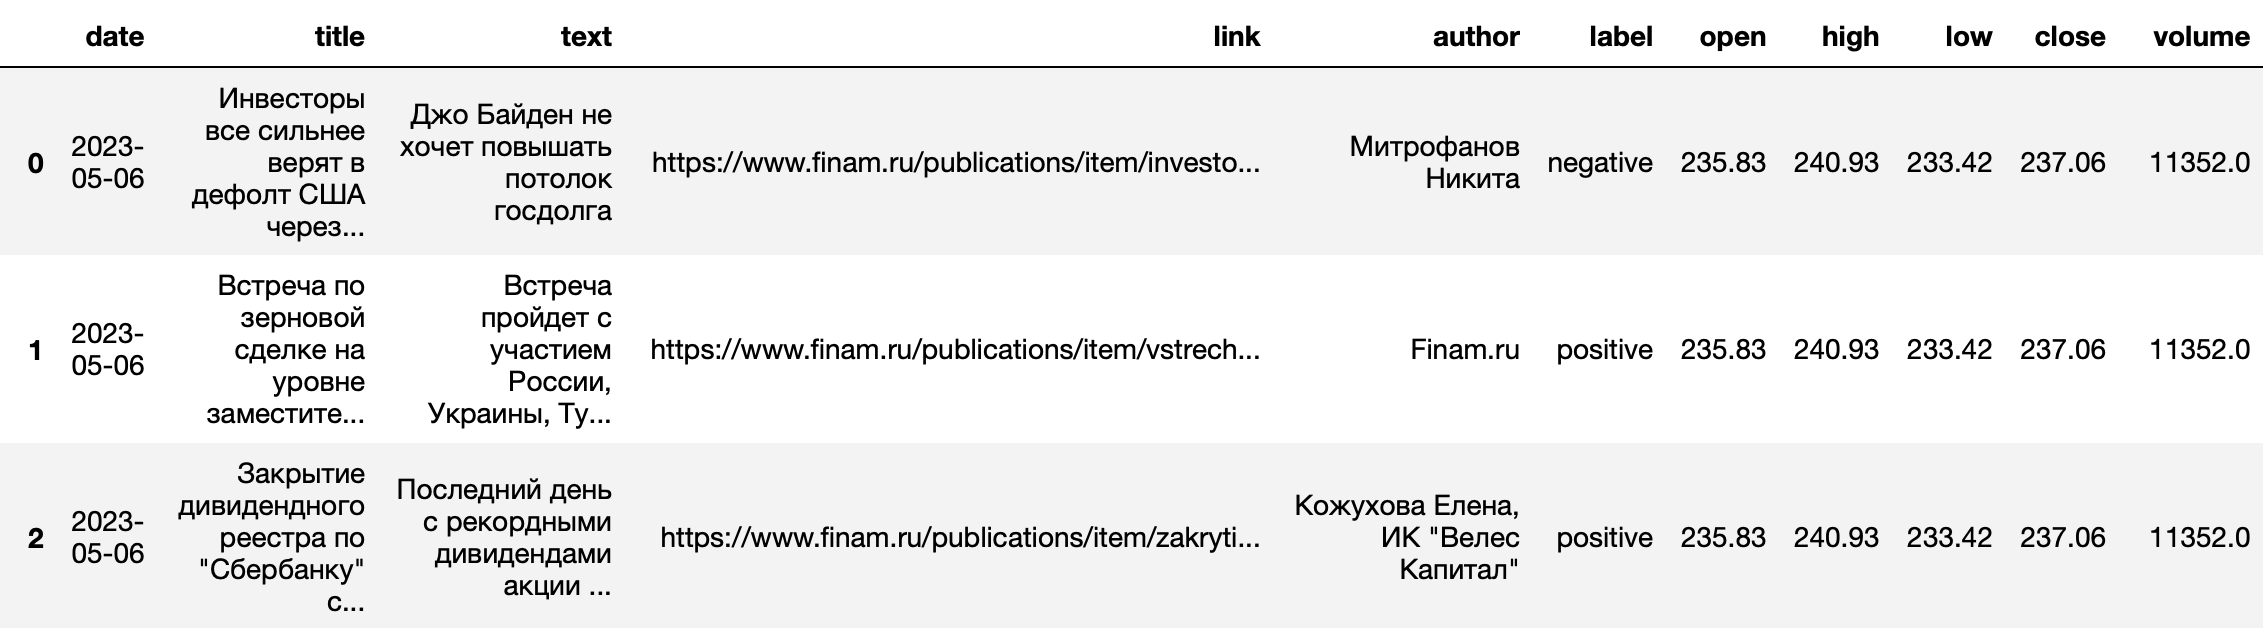
\includegraphics[width=0.9\linewidth]{dataset.png}
    \caption{Dataset samples represented as DataFrame.}
    \label{fig:dataset}
\end{figure}

I represent some statistics of resulting StocksNews dataset on Tab.~\ref{tab:statistics} The dataset was split into two parts: train and test with proportion of 88/22 percent accordingy. It's important to mention that this is a time series dataset so I did not use any kind of shuffling. 

\begin{table}[tbh!]
\begin{center}
\begin{tabular}[t]{|l|c|c|}
\hline
%\cline{2-4}
 & Train & Test \\
\hline
\hline
Proportion & 0.88 & 0.22  \\
\hline
Size & 23879 & 6735 \\
\hline
Vocabulary size & \multicolumn{2}{c|}{16507} \\
\hline
Date range & 2022.05.08 - 2023.02.10 & 2023.02.10 - 2023.05.06 \\
\hline
\end{tabular}
\caption{Statistics of the StocksNews dataset.}
\label{tab:statistics}
\end{center}
\end{table}

\begin{figure}[!tbh]
    \centering
    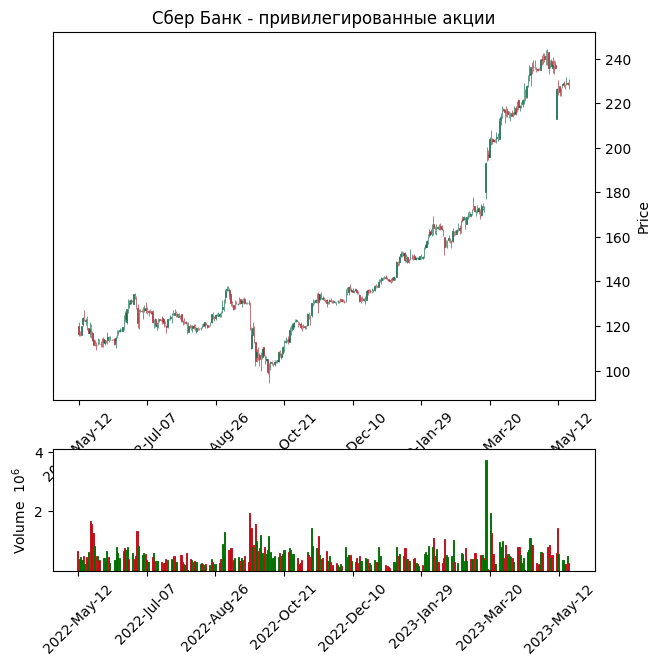
\includegraphics[width=0.9\linewidth]{sber.png}
    \caption{Sberbank shares cost values in dataset.}
    \label{fig:sber}
\end{figure}

When constructing a baseline with TF-IDF\footnote{TF-IDF model to get the sentence embeddings. Details at ~\href{https://ru.wikipedia.org/wiki/TF-IDF}{Wikipedia} or in work by \cite{Ramos1999}.} embeddings, I have used lowercase sentences, \texttt{mystem} for lemmatizaton, \texttt{nltk} for stopwords filtering.

It's worth mentioning that use of other dataset preprocessing techniques have not been done. It could be a topic for other possible research which is out of scope of current.

For implementing a related work solutions I have labeled every sentence with one of four sentiment labels which was correct in my personal opinion as a novice investor. The distibution of labels is shown of Pic. ~\ref{fig:labels}

\begin{figure}[!tbh]
    \centering
    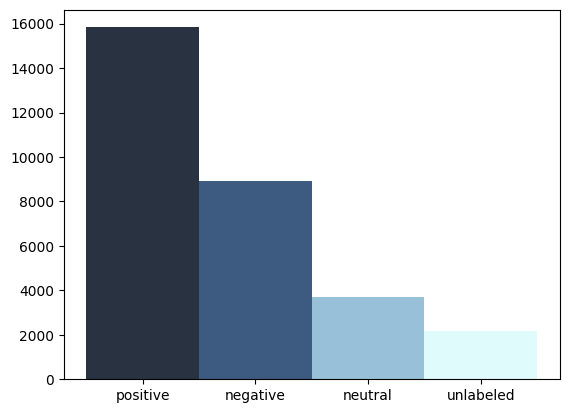
\includegraphics[width=0.5\linewidth]{labels.png}
    \caption{Distribution of sentiment labels in dataset.}
    \label{fig:labels}
\end{figure}



\section{Experiments}
\label{sec:experiments}
\subsection{Metrics}
The evaluation of every solution was scored by 2 types of metrics: regression and classification metrics.
My goal was not only to see how close the forecast is to real data via checking regression metrics score, but also to check whether the predictions are correct in the terms of market change direction. And see if you can rely on it during trading.
For that I have used classification metrics.

Following sections contains $\hat{y}$ and $y$ as a forecast values and actual values respectively.

\paragraph{Regression metrics}

The first is Mean Squared Error:
\begin{align}
MSE(y, \hat{y})=\sum_{i=1}^{D}(y_i-\hat{y}_i)^2,
\end{align}
this metric was chosen to have a general sense of how close the forecasts are.

For intuitive interpretation the Mean Absolute Percentage Error was used:
\begin{align}
{MAPE(y, \hat{y})={\frac {100\%}{n}}\sum _{t=1}^{n}\left|{\frac {y_{t}-\hat{y}_{t}}{y_{t}}}\right|}
\end{align}
\paragraph{Classification metrics}

The accuracy was also used to have a comprehension of models correct choices. I named it as Stock Option Accuracy Score:

\begin{align}
SOAS(y, \hat{y}) = ACC(z, \hat{z}),
\end{align}
\begin{align}
where \quad ACC(z, \hat{z}) = \frac{\left|\{z_i == \hat{z}_i \mid i = 0...n\}\right|}{n}, \nonumber 
\end{align}
 \begin{align}
    where \quad z_{i} = \begin{dcases*}
        1, & if $ y_{i+1} - y_{i} > 0 $,\\
        0, & otherwise. 
        \end{dcases*} \nonumber 
  \end{align}
 \begin{align}
    where \quad \hat{z}_{i} = \begin{dcases*}
        1, & if $ \hat{y}_{i+1} - \hat{y}_{i} > 0 $,\\
        0, & otherwise. 
        \end{dcases*} \nonumber 
  \end{align}


I also came up with a metric called Stock Possible Profit Percent Score or S3PS for short:
\begin{align}
S3PS(y, \hat{y}) = 100 * [\prod_{i=0}^{n-1}{(1 + C_i)} - 1],
\end{align}
\begin{align}
where \quad C_i = \begin{dcases*}
        P_i, & if $ y_{i+1} - y_{i} > 0  \quad and \quad \hat{y}_{i+1} - \hat{y}_{i} > 0 $,\\
        P_i, & if $ y_{i+1} - y_{i} <= 0  \quad and \quad \hat{y}_{i+1} - \hat{y}_{i} <= 0 $,\\
        -P_i, & otherwise. 
        \end{dcases*} \nonumber 
\end{align}
\begin{align}
where \quad P_i = \left| 1 - (y_{i+1}/y_{i}) \right| \nonumber 
\end{align}

It is based on SOAS but represents possible percentage gain if we follow a strategy suggested by model.


\subsection{Experiment Setup}
I setup the experiment and train the proposed model for 5000 episodes (epochs).
The hyperparameters are show in Tab.~\ref{tab:hyperparams}
It was convinient to run training procedure in jupyter notebook, so I represented learning algorithm on the graph as shown in \texttt{/notebooks/lstm-gym-embeddings.ipynb}

I also experimented with bert embeddings using sentence transformers and \href{https://huggingface.co/cointegrated/rubert-tiny}{rubert-tiny} pretraind model.

\begin{table}[tbh!]
\begin{center}
\begin{tabular}{ |r||c|l|  }
 \hline
 \multicolumn{3}{|c|}{Hyperparameter List} \\
 \hline
 Param Name & value & description \\
 \hline
 $BATCH-SIZE$   & 128    & bathes from the replay buffer\\
 $FAIL-DIFF$ & 0.05 & max agent deviation to terminate env\\ 
 $DIFF-REWARD$ & 0.001 & how close agent should be to the target to get a reward\\
 $SEQUENCE-LEN$ & 42 & length of data for previous days  \\
 $GAMMA$   & 0.99    & discount factor\\
 $EPS-START$ & 0.9    & start of epsilon\\
 $EPS-END$ &  0.05    & final value of epsilon\\
 $EPS-DECAY$ &  1000    & rate of exponential decay\\
 $TAU$ &  0.005    &update rate of the target network\\
 $LR$ &  1e-4    &learning rate\\
 \hline
\end{tabular}
\caption{Hyperparameters of proposed method.}
\label{tab:hyperparams}
\end{center}
\end{table}


\subsection{Baselines}
\label{sec:baseline}
First of all I implemented a baselines with TF-IDF embeddings and multiple linear or non-linear methods over it. 
I got some results to start with and some functions which helped me in the future solutions.
For more info, please visit a \texttt{/notebooks/baseline.ipynb}

\section{Results}
\label{sec:results}

In the Tab. \ref{tab:results} I refer to achieved results and provide brief conclusions.

\begin{table}[tbh!]
\begin{center}
\begin{tabular}{ |c||c|c|c|c|  }
 \hline
 \multicolumn{5}{|c|}{Results comparison} \\
 \hline
 Method Name & MSE & MAPE & SOAS & S3PS \\
 \hline
 \hline
 RIDGE & 1253.37 & 0.12 & 0.44 & 4.85\% \\
 \hline
 TREES & 3919.90 & 0.25 & 0.46 & -14.12\% \\
 \hline
 LSTM & 155.04 & 0.04 & 0.41 & 4.24\% \\
 \hline
 DQNFCN & 2027.74 & 0.20 & 0.44 & -9.75\% \\
 \hline
 DQNLSTM & 166.67 & 0.05 & 0.56 &  7.33\% \\
 \hline
\end{tabular}
\caption{Results of all methods of research.}
\label{tab:results}
\end{center}
\end{table}

In the course of experimenting I implemented a prototype for each solution and graphical representation for better understanding of the results.

A baselines are good starting points, because some of them have reached the FCN proposed solution.

Even though the proposed model did not overcome the LSTM by \cite{Sen_2021} in regression metrics, it showed a decent results in classification metrics.
S3PS metric shows how much percent we could possibly gain when following a strategy. 
With that being said, it means the reinforcement learning techniques can be useful for solving a human-like tasks, including trading.

The sample of model forecast results could be found in Fig.~\ref{fig:forecasts}.

\begin{figure}[!tbh]
    \centering
    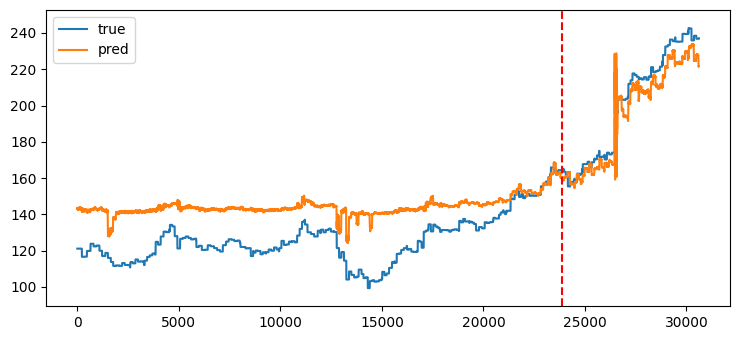
\includegraphics[width=0.9\linewidth]{forecasts.png}
    \caption{Price forecast split by red dashed line.}
    \label{fig:forecasts}
\end{figure}

\section{Conclusion}
It was quite interesting research for me, I have managed to make my own dataset\ref{sec:dataset}, solved the task with baselines\ref{sec:baseline}, implement available solutions using research reports which were mentioned in section\ref{sec:related}, explore \href{https://pypi.org/project/gymnasium/}{gymnasium}  deep q-learning framework, and make my own RL environment where i did all the experiments \ref{sec:experiments}

It's worth mentioning that there are plenty of other research possibilities left out of scope of current work, including hyperparameter tuning, model ensembles, different architectures, also sources of news articles, text preprocessing, other companies shares and so on.

To conclude, reinforcement learning is a powerful machine learning technique that has shown great promise in solving complex real-world problems.

\bibliographystyle{apalike}
\bibliography{lit}
\end{document}
